\documentclass{article}
\usepackage{graphicx} % Required for inserting images
\usepackage{url}
\usepackage{hyperref}
%\usepackage{natbib}
\usepackage{verbatim}
\usepackage{natbib}
\usepackage{amsmath} 
\usepackage{xcolor}

\hypersetup{colorlinks=true,citecolor=blue}
\hypersetup{colorlinks=true,linkcolor=blue}
\hypersetup{colorlinks=true,urlcolor=blue}

\usepackage[letterpaper,top=3cm,bottom=3cm,left=4cm,right=4cm,marginparwidth=1.75cm]{geometry}

\begin{document}

\title{Higher Education Access Disparities in Portugal}
\author{Miguel Sousa Duarte\thanks{{\tiny{}Department of Economics, Copenhagen Business School. \textbf{E-mail}: \url{msd.eco@cbs.dk}.}},
Vicente Conde Mendes\thanks{{\tiny{}École Polytechnique Fédérale de Lausanne. \textbf{E-mail}: \url{vicente.c.mendes@gmail.com}.}}\\}

\date{\today}

\setlength{\parskip}{1em}
\maketitle

\section{Introduction}
While private school students in Portugal tend to outperform their public school peers on both internal grades and national exams, they also experience greater grade misalignment — meaning the gap between their school-given grades and their exam results is wider. If university admissions rely on inflated internal grades, private school students may benefit disproportionately. In this study, we quantify grade inflation across schools and its impact in the access to higher education. 

In Portugal, 25\% of high school (HS) students attend private institutions (Pordata, 2022). In general, private HS, which can select which students to admit into their alumni, are fully-funded by the tuition they charge their students. As such, on average, students in private HS come from a more privileged socioeconomic background. Parents choosing to enroll their children in a private school likely value the quality of education provided. Nonetheless, other incentives may be at play. In Portugal, graduation from high school is conditional on passing standardized national exams (NE) on some of the subjects the students took during HS. The HS grade-point average (GPA) for applying to public university then is a weighted average of both NE and school-internal grading. We, thus, believe there is room for schools to, not the least following pressure exerted by paying parents, inflate grades and, hence, improve the chances of admission to top public university programs, the most competitive in the country.

The problem at hand is not applicable to all countries. First, there are countries with university-specific admission tests, e.g. Italy, where the weighting on internal grading is limited. Second, some countries, like the Netherlands, opt for enrolling a big mass of students into a, typically harder, 1st year of the studies, which then allows for a natural selection process once at the university, as the less able students drop out of the programs. Third, in countries where admissions are application-based, such as the US, the Admissions committee of each university, aimed at enrolling the best students, can factor in school-specific grade inflation when selecting applicants. Several other countries, such as Denmark (quota 1), Slovenia, Sweden, Spain and Norway are, however, subject to similar grade-dependent admissions process, where such issues may arise. Nonetheless, few of them have such a widespread system of private schools whereby moral hazards may arise.

This is a topic that generates strong emotions because, if it occurs, it constitutes a profound injustice, given the decisive role that internal grades play in access to higher education in the country. The key questions are whether grade inflation is in fact real and whether it has a measurable impact on university admissions. Furthermore, does this practice differ clearly between private and public schools, or is it more closely associated with specific regions? To address these questions, we analyzed data made available by Directorate-General for Statistics of Education and Science (in Portuguese, DGEEC) encompassing all students taking national exams in the period 2014 - 2023 in order to arrive at an objective answer.

In this essay, we present our preliminary findings, which reveal a recurring practice of grade inflation in certain schools — an outcome that represents a serious injustice in the process of accessing higher education. Because our aim is not merely to highlight shortcomings but also to point toward remedies, we conclude by discussing possible solutions. That said, it is important to underline the qualitative distinction between the two parts of this essay: in the main body, where we describe the problem, our argument rests on factual evidence—grade inflation demonstrably exists in many schools in Portugal, and this can be shown empirically. In the concluding section, however, our focus turns to potential reforms, which necessarily involve personal judgment and opinion. Here our intention is to open a space for discussion and to actively invite contributions with alternative or better ideas than our own. Without further delay, we begin with a technical introduction, which may be skipped by those interested solely in the results and conclusions.

\section{Technical Introduction}
\label{sec:TechnicalIntroduction}

The starting point of our analysis is the simplest and most objective measure to study grade inflation, which we will refer to as grade misalignment\footnote{This follows the Portuguese Ministry of Education terminology: \textit{desalinhamento de nota}}:
\[
\text{Grade Misalignment} = \text{Internal Grade} - \text{NE grade}
\]  
This measure is only well defined for subjects subject to a NE. It is calculated for all exam–internal grade pairs in the dataset. Unless stated otherwise, the entire discussion that follows is restricted to these subjects, for which we possess a clear measure of grade inflation. This is possible because we can use performance on the national examination — identical for all students in the country, regardless of their school.

\textcolor{red}{Following part should show the same but our own results! Problem: We do not export it separately, just the difference}

\textcolor{gray}{Private schools' students score, on average, 4.1 points below on their national exams compared to their school-given grade (Figure \ref{fig: InflationBySchoolType}). For public schools, this gap is of 3.7 points. In fact, as stated by \cite{sapo2024}, the ten 10 HS with the greater difference between internal grading and NE grade are private.
If national exams are a good measure of true ability, then private schools inflate their students' grades by 10\% than public schools. This provides an unfair advantage to private HS students.}

\begin{figure}[ht]
  \centering
  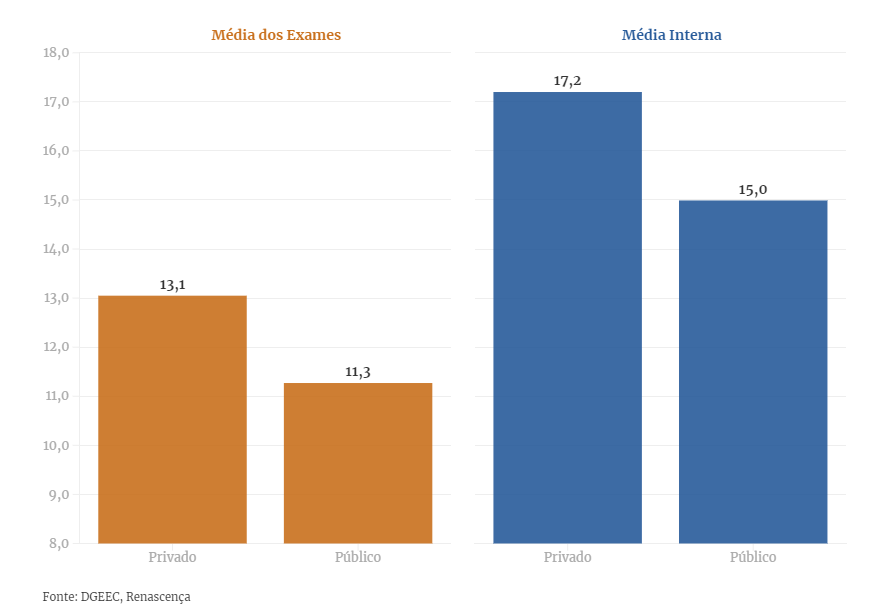
\includegraphics[height=4.3cm, keepaspectratio]{Figures/InflationBySchoolType.png}
  \caption{Grade Misalignment by School Type \citep{sapo2024}}
  \label{fig: InflationBySchoolType}
\end{figure}
%add source


Private HS students achieve higher grades both on school-internal grading and on National Exams (NE) when compared to public HS students. This can be due to several reasons, among them, 1) private HS students' innate ability is better; 2) private HS students have access to better outside-of-the-classroom resources; 3) the education provided by private schools is better. Reason 1) may cause backlash but it is not implausible that ability of parents is correlated with ability of children and that ability of parents is correlated with income of parents. Reason 2) derives from the plausible assumption that having the means and willingness to pay for private education positively correlates with having the means and willingness to pay for tutoring. As for reason 3) it is widely recognized in Portugal that private HS tend to provide a better education than their public counterparts - even though reasons 1 and 2 may contribute towards the overall societal perception of the gap in education quality.
Nonetheless, it seems agreeable to conclude that private HS students in Portugal are privileged. 

%Simpson's Paradox

Private schools have students who perform better both on internal and external grading. While the global average shows that private schools' grade misalignment is only 10\% than public schools, there are reasons to take this gap seriously. As there is a upper bound on the school grade (20), lower grades are bound to having more inflation. A Simpson's Paradox then emerges as public schools have more individuals with low grades. This means that public schools seem more inflated if the analysis is not made conditional on grade.


To address this paradox, we follow the approach of \cite{nata2014unfairness}, grouping students according to the ten-point interval of their score on the NE. For each group of schools, we then compute and plot the average grade misalignment, as shown in Figure \ref{fig:inflacao_bins_pub_priv_en}. The figure reveals that, across all NE score ranges, private high schools consistently exhibit a larger differential. This pattern provides strong evidence of systematic grade inflation within private institutions.


\begin{figure}[ht]
  \centering
  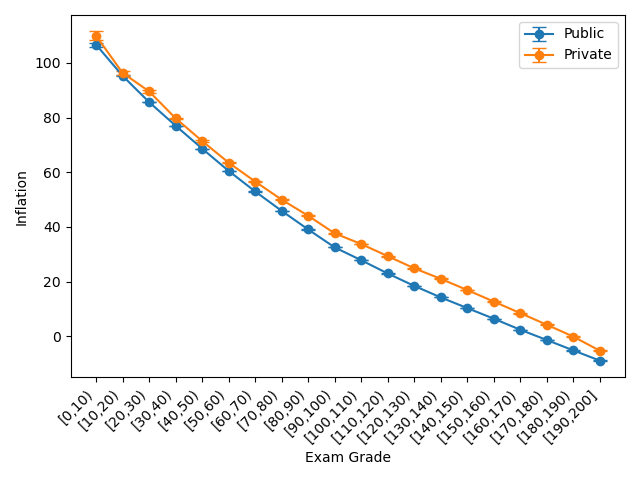
\includegraphics[height=7cm, keepaspectratio]{Figures/inflacao_bins_pub_priv_en.png}
  \caption{Grade Misalignment plotted against NE grade }
  \label{fig:inflacao_bins_pub_priv_en}
\end{figure}

% Introduce new/adjusted inflation measure

\subsection{Regression}
\label{sec:regression}

In spite of the existence of the grade misalignment measure, we are going to be discussing inflation. Inflation represents how much higher/lower the internal grade is compared to what’s predicted by the exam grade. For this purpose, we present a simple OLS regression:

\begin{equation}
GM_{i,s} = \alpha + \beta \, G^{\text{exam}}_{i,s} + \varepsilon_{i,s} \nonumber
\end{equation}

The dependent variable is grade misalignment (GM) and the dependent variable is the exam grade ($G^{exam}$). The subscripts $i$ and $s$ identify students and schools respectively. The $\alpha$ coefficient represents the grade misalignment that is expected, regardless of the school attended or grade achieved. As seen at the beginning of Section \ref{sec:TechnicalIntroduction}, internal grade is on average much larger than external grade across both school types. As such, one expects $\alpha$ to be positive. What cannot be explained by the exam grade - a proxy for true ability - is then part of the error term $\varepsilon_{i,s}$. Having computed the coefficients of the regression, we subtract the fitted values $\hat{\alpha} + \hat{\beta}  \, G^{\text{exam}}_{i,s}$ to obtain fitted residuals:

\begin{equation}
\hat{\varepsilon}_{i,s} = GM_{i,s} - \left( \hat{\alpha} + \hat{\beta}  \, G^{\text{exam}}_{i,s} \right) \nonumber
\end{equation}

School-specific inflation then is given by the average of the fitted residuals of all students in a certain school:

\begin{equation}
\widehat{\text{Inf}}_{s}
= \bar{\hat{\varepsilon}}_{s}
= \frac{1}{n_s}\sum_{i \in s}\hat{\varepsilon}_{i,s} \nonumber
\end{equation}




\textcolor{red}{Here, I would introduce Literature Review, Institutional Details and Data. For the paper, they must all be there. For this piece, I would maybe have one line about \citep{nata2014unfairness}, and then one paragraph on Institutional Details and Data, mainly focused on explaining CNA process. Let's discuss it. For now, I skip it altogether.}

\section{Inflation Analysis}
We now dive deeper into comparing how inflation differs across schools. We start by understanding the degree of recidivism of schools: are there some schools that consistently exhibit a pattern of higher differential? For this purpose, Figures \ref{fig:HeatmapPublicNoMissing} and \ref{fig:HeatmapPrivateNoMissing} display heatmaps where each row represents a school (code) and each column a school year (2020 and 2021 ommited due to lack of data following rule changes in Covid period). The graph thus ought to be read horizontally as one compares the level of inflation observed in a certain school across years. \textcolor{red}{Here, it is not obvious to me that there is greater recidivism in private schools. So, still need to add interpretation here. Will do when new data is available.}

\begin{figure}
    \centering
    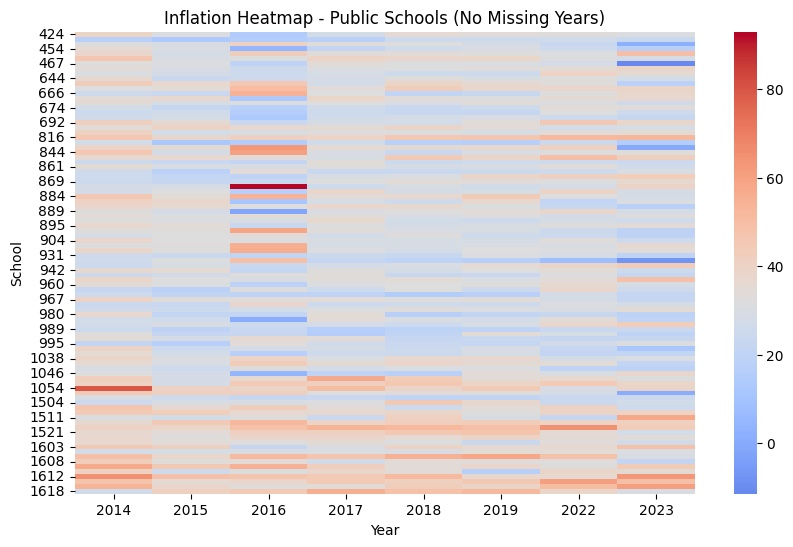
\includegraphics[width=0.8\linewidth]{Figures/HeatmapPublicNoMissing.jpeg}
    \caption{Inflation Heatmap - Public Schools}
    \label{fig:HeatmapPublicNoMissing}
\end{figure}

\begin{figure}
    \centering
    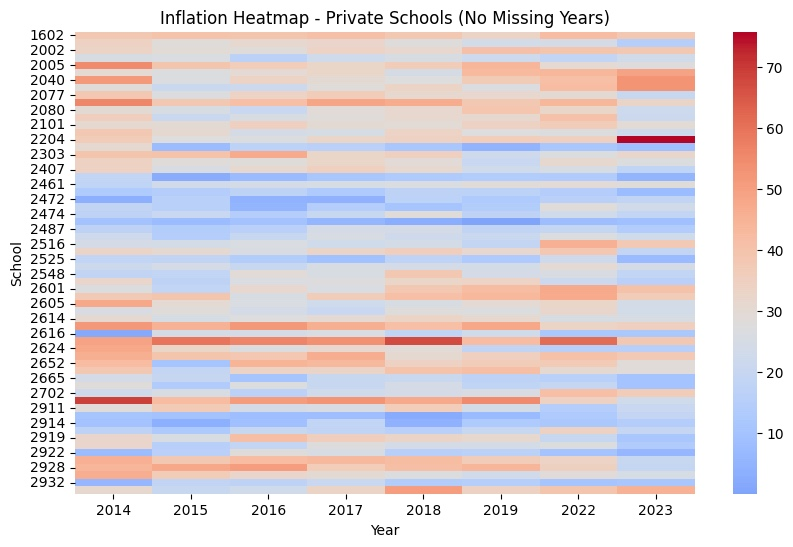
\includegraphics[width=0.8\linewidth]{Figures/HeatmapPrivateNoMissing.jpeg}
    \caption{Inflation Heatmap - Private Schools}
    \label{fig:HeatmapPrivateNoMissing}
\end{figure}

Next, we explore the distribution of these differentials, within private and public schools. Figure \ref{fig:DistributionInflationPublicPrivate} shows the histogram for school inflation across public and private schools. Inflation is  generalized for both types of school. The mean is not fundamentally different across groups, however, we see that across private high-schools (orange), the variance of the differential is much higher than across public schools. Given the more widespread distribution of inflation across private schools, let us think about the whole sample as being composed of three groups in ascending order of grade inflation: well-behaved private, public and misbehaving private. 

Well-behaved private schools are generally located to the left of the bulk of public schools (blue), with students who achieve top marks in both internal assessments and national exams. These schools exhibit low inflation -- partly constrained by the grade ceiling -- and their students legitimately secure places at the most competitive universities. Public schools also display some degree of grade inflation, but it is relatively uniform across this sector. At the other extreme are the misbehaving private schools, situated in the right tail of the private school distribution.

Our hypothesis is that while students from public schools do not displace their peers from well-behaved private schools, the situation changes in the case of misbehaving private schools. Here, substantial grade inflation artificially boosts students’ application GPAs, enabling them to gain admission ahead of equally capable public school peers. In contrast, private schools with only moderate misalignment—where high-achieving students receive strong but not excessively inflated grades—offer little scope for such unfair displacement. The real concern, therefore, lies with the subset of private schools that systematically inflate grades far beyond the norm.

\begin{figure}
    \centering
    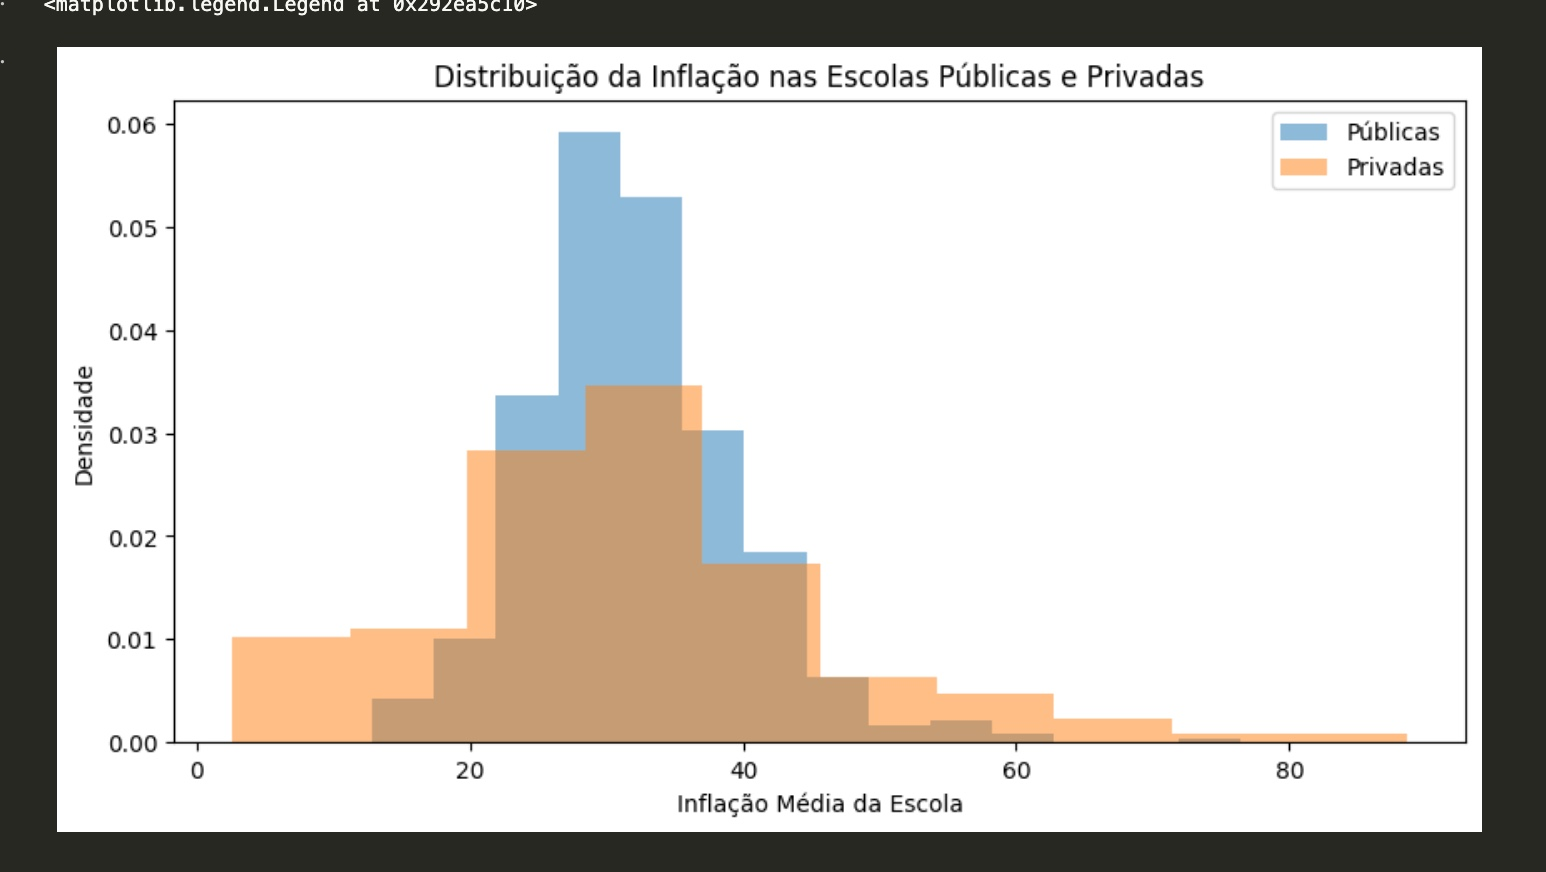
\includegraphics[width=0.75\linewidth]{Figures/DistributionInflationPublicPrivate.jpeg}
    \caption{Distribution of Average School Inflation across School Types}
    \label{fig:DistributionInflationPublicPrivate}
\end{figure}


\section{Outros - Inf por disciplina, por distrito, disciplinas sem exame}

One of the limitations of our method, is that some subjects, which are not subject to NE - or at least not mandatorily so - do not allow for this analysis, as they lack the less biased grade from a standardized examination. Nonetheless, policy can introduce exogenous variation that allows for studying potential inflation in grades not subject to NE. In Portugal, the grade obtained in Physical Education (PE) stopped counting for higher education application GPA in the period 2012 - 2018, after which it was re-introduced. It is thus possible to compare the grades that schools were awarding before and after the halt in PE grade counting was lifted. The validity of this analysis thus lies behind of the assumption that average ability of students in a school should not change upon the policy change, which we believe to be valid, as contrary to the US, there is no sport-oriented recruitment done at the HS level. PE is particularly interesting because there is less reason to believe that private students should be more able at it, as happens with more 'academic' subjects.



\section{Discussão what else could be done}

\begin{enumerate}
    \item Having been able to identify the level of inflation across schools, one is left to wonder as to the true impact of this phenomenon. This motivates our next task: running a counterfactual experiment, where the admission algorithm is re-run with inflation-adjusted grades. This is made possible due to a centralized admission process of students to public higher education. Students rank their preferred university-programme pairs of choice in a list with a maximum of 6 elements. Admission follows a deferred acceptance algorithm exclusively dependent on the GPA with which the student concluded High School and on the grades scored on the NE. Generally, the application grade is the arithmetic mean of the school-given internal grade and the grades scored on the NE relevant for the Bachelors programme (exact proportion and which NE are relevant are defined by the university). The key factor here is that the schools' internal grading play a relevant role in university application GPA, in a system in which this is the only qualifying mechanism.
    At this stage, we are awaiting access to the data on the choice of HS graduates for public Higher Education made on the National Access Contest (in Portuguese, CNA) before being able to perform the simulation.

    \item In the Covid period, rules regarding mandatory NE became more lenient: students only had to take exams they wanted to use for accessing Higher Education. The attenuating effect of the NE counting for the internal grade was therefore weaker during this period for some of the subjects. Furthermore, exams were easier, graded out of 20 but with 20+ possible points. A higher rate of students getting a perfect score puts more emphasis on internal grading in distinguishing the students. Both of these points are concerning. Though our external grading sample for comparison decreases, it may be useful to make a comparison across different year-cohorts in the same school to see whether teachers inflated grades further given that, during this period, there was no NE grade to compare the students' school performance to.

\end{enumerate}




\section{Discussão soluções}


\section{Conclusão}

Our work is motivated by the unfair advantage that private high school students hold over their public school peers when applying to higher education. This advantage arises from more favorable internal grading, which directly contributes to the university application GPA—the central criterion for admission. In addition, these students tend to come from more advantaged socioeconomic backgrounds, which provides greater support outside the classroom.

We argue that comparing average grade inflation between public and private schools obscures important differences. In fact, private schools display a much wider dispersion in inflation. At one end, some private schools are “well-behaved,” inflating as little as (or even less than) the least-inflating public schools. At the other end, however, the most extreme cases of inflation are concentrated among private schools: the ten highest-inflating schools are all private \citep{sapo2024}. %this citation should go away.

Our interpretation is that well-behaved private schools generally serve high-achieving students whose strong exam performance naturally results in low inflation. For such students, inflation is further constrained by the upper bound of 20 on internal grades. Public schools, by contrast, exhibit more uniform levels of inflation. Their averages are often driven upward by lower-performing students who manage to pass internally but subsequently perform poorly in national exams. To focus on the group most relevant for competitive admissions, we restrict attention to students with internal grades between 14 and 20, as these are the individuals most likely to be competing for places in public universities. Finally, we identify a subset of “misbehaving” private schools that inflate grades far more aggressively than the rest. These schools drive up the private-sector average and likely produce the students who benefit most from the system, potentially displacing equally or more capable students from public schools.

Our next contribution will be to adjust students’ GPAs according to the inflation level observed in their schools, re-run the university placement algorithm, and compare the adjusted outcome with the official assignment. If the most able students are not securing the most competitive places under the current system, this would provide clear evidence of inefficiency and unfairness in admissions.



\bibliographystyle{apalike}
\bibliography{references}

\newpage
\appendix
\section{Regression with Polynomial}

If the regression is ran using a cubic polynomial in the exam grade, then the Section \ref{sec:regression} equations are as follows:

\begin{equation}
GM_{i,s} = \alpha 
+ \beta_1 \, G^{\text{exam}}_{i,s} 
+ \beta_2 \, \left(G^{\text{exam}}_{i,s}\right)^2
+ \beta_3 \, \left(G^{\text{exam}}_{i,s}\right)^3
+ \varepsilon_{i,s} \nonumber
\end{equation}

\begin{equation}
\hat{\varepsilon}_{i,s} = GM_{i,s} 
- \left( \hat{\alpha} 
+ \hat{\beta}_1 \, G^{\text{exam}}_{i,s} 
+ \hat{\beta}_2 \, \left(G^{\text{exam}}_{i,s}\right)^2
+ \hat{\beta}_3 \, \left(G^{\text{exam}}_{i,s}\right)^3 \right) \nonumber
\end{equation}

\begin{equation}
\widehat{\text{Inf}}_{s}
= \bar{\hat{\varepsilon}}_{s}
= \frac{1}{n_s}\sum_{i \in s}\hat{\varepsilon}_{i,s} \nonumber
\end{equation}


% \renewcommand{\thefigure}{A\arabic{figure}} % Change figure numbering to A1, A2, etc.
% \setcounter{figure}{0} % Reset figure counter

% \begin{figure}[ht]
%   \centering
%   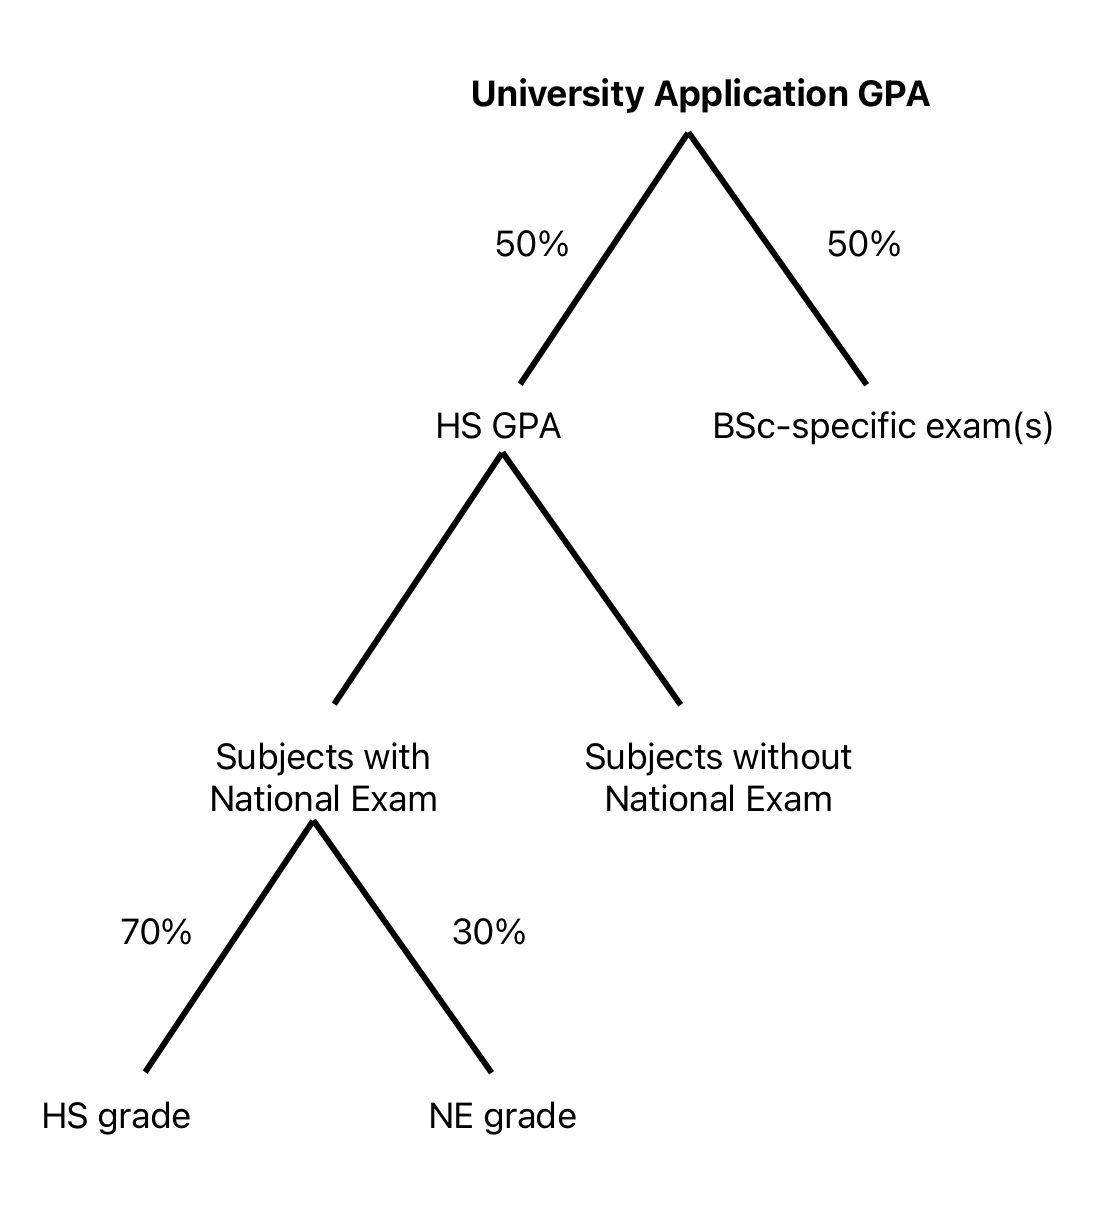
\includegraphics[height=10cm, keepaspectratio]{Figures/GradeComputationPortugal.jpeg}
%   \caption{GPA Computation Rules in Portugal}
%   \label{fig: GradeComputationPortugal}
% \end{figure}

\end{document}